\section*{Question 1.1 - Sieve of Eratosthenes - MPI (Single Machine)}

In this question we were asked to rewrite our earlier implementation of the 
Sieve of Eratosthenes using MPI, while utilizing `MPI\_send` and `MPI\_Recv`. 
Once complete we were then asked to run the code on a single server and note the 
speed-up/slow-down when compared to previous implementations.

\subsection*{Process}

\begin{itemize}
\item Reusing our implementation of the sieve from Assignment 2, we first 
removed all PThread specific code.
\item Proceeded to the add in the required MPI directives.
  \begin{itemize}
    \item MPI\_Init
    \item MPI\_Comm\_rank
    \item MPI\_Comm\_size
    \item MPI\_Send
    \item MPI\_Recv
  \end{itemize}
\item Once the code was refactored with the correct directives, testing of the 
code then began.
\item Once satisfied that the code still functioned as expected (and produced 
the correct results) we then began testing and recording the data.
\end{itemize}

\subsection*{Difficulty}

When comparing to the PThread implementation, using MPI was far easier to write. 
However using OpenMP far exceeds MPI in ease-of-use, readability and code-length.

\subsection*{Results}

\begin{figure}
  \centering
  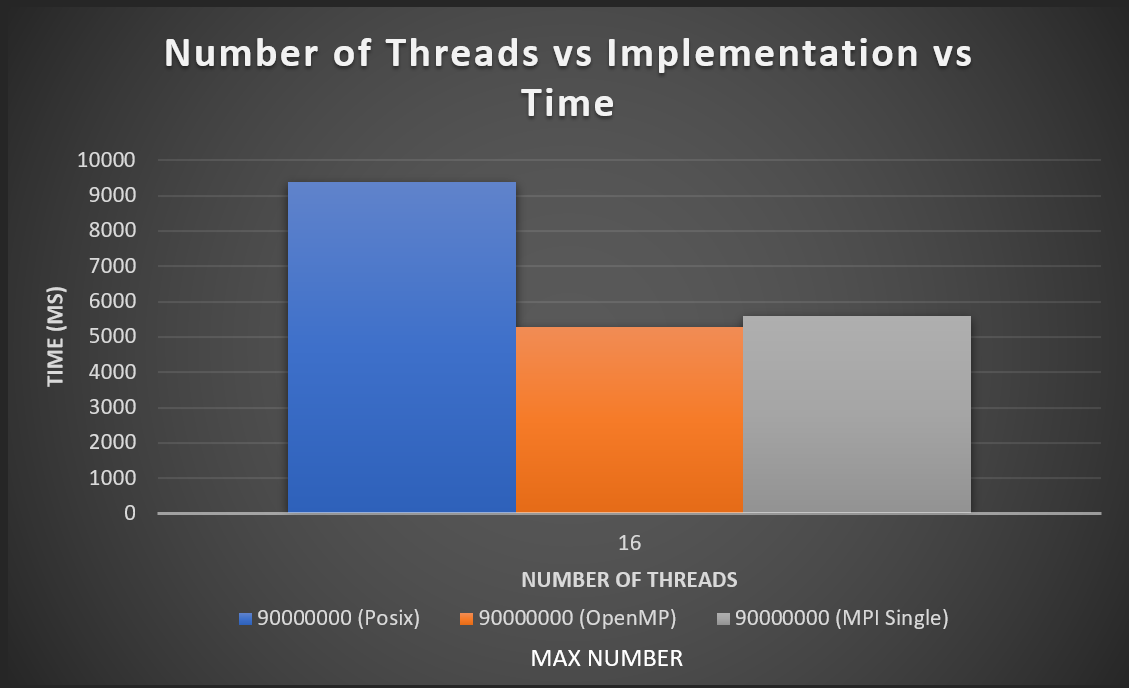
\includegraphics[width=\linewidth]{Figures/mpi_SINGLE.png}
  \caption{Sieve of Eratosthenes with max number $9\times10^7$ on different
  implementations.}
  \label{fig:sievesingle}
\end{figure}

As seen in figure\ref{fig:sievesingle}, running the MPI implementation on a single machine far 
outstripped our initial PThread version with about a ~50\% reduction in time.
However when compared to the OpenMP implementation, we see that the MPI version 
is slightly slower. This seems to be likely due to the manual calculation of the 
`range`, `startNumber` for each thread (we assume that that OpenMP's `for` 
directive has a far more refined and optimized algorithm than ours).
